\documentclass[12pt, titlepage]{article}

\usepackage{amsmath, amssymb}
\usepackage[margin=0.75in]{geometry}

\usepackage{subcaption}
\usepackage{graphicx}
\graphicspath{{./img/}}

\usepackage{listings}
\usepackage{color}
\definecolor{mygreen}{rgb}{0,0.6,0}
\definecolor{mygray}{rgb}{0.5,0.5,0.5}
\definecolor{mymauve}{rgb}{0.58,0,0.82}

\lstset{ 
  backgroundcolor=\color{white},
  basicstyle=\footnotesize\ttfamily,
  breakatwhitespace=false,
  breaklines=true,
  captionpos=b,
  commentstyle=\color{blue},
  extendedchars=true,
  frame=tb,
  keepspaces=true,
  keywordstyle=\color{mymauve},
  numbers=left,
  numberstyle=\footnotesize\ttfamily\color{mygray},
  rulecolor=\color{black},
  showspaces=false,
  showstringspaces=false,
  showtabs=false,
  stepnumber=1,
  stringstyle=\color{mygreen},
  morestring=[d]",
  tabsize=2,
  title=\lstname
}

\lstdefinestyle{cypher}{
  morekeywords={CREATE, MATCH, WHERE, RETURN, AND, IN},
}

\lstdefinestyle{mql}{
  morekeywords={
    WHO,
    WHEN,
    WHAT,
    WHERE,
    DESCRIPTION,
    head,
    parent,
    branchName,
    active,
    timestamp,
    created
  }
}

\renewcommand{\refname}{Références}

\title{\textbf{IFT4055 - Projet Honor} \\ MQL à Cypher -- Un Framework pour
  Traduire un Langage de Requêtes Spécifique au Domaine pour Interroger un
  Projet Versionnable en des Expressions Cypher}
\author{Philippe Gabriel - 20120600}
\date{18 décembre 2022}

\begin{document}

\maketitle
\pagenumbering{arabic}
\setcounter{page}{2}

\section*{Problème}

Les systèmes de versions de contrôle (\textit{Version Control System} -- VCS)
présentent une grande importance dans les besoins de vouloir gérer le
versionnement de collections de données. Dans le domaine de l'informatique et de
l'ingénierie logicielle, des systèmes comme Git représentent une très grande
importance dans la pratique menant à l'intérêt industrielle du développement de
grands logiciels. L'ingénierie dirigée par les modèles (\textit{Model-Driven
Engineering} -- MDE) est une approche présentant plusieurs avantages dans la
conception de logiciels. Cette approche permet au concepteur d'abstraire des
détails des langages de programmation générals, de sorte à concentrer ses
efforts dans la résolution du problème. L'usage de modèles ou de langages
spécifiques au domaine (\textit{Domain-Specific Languages} -- DSL) aide l'expert
à s'exprimer dans une terminologie propre à son domaine d'étude et lui
permettrait de contribuer à la conception d'un logiciel sans avoir de
connaissances de programmation. Un intérêt industrielle commence à se manifester
pour la MDE poussant à l'adopter pour concevoir de larges projets. Un VCS
orienté-ligne comme Git utilisé pour gérer le versionnement des changements
apporter à un projet MDE n'est pas la meilleure approche à adopter gérer de gros
projets. L'interprétation des changements sur un modèle conçu par l'expert du
domaine sera au niveau de la sérialisation du modèle. Cette interprétation n'est
donc pas spécifique au domaine du modèle. La sémantique riche du domaine est
complètement négligé. Un VCS spécifique au domaine (\textit{Domain-Specific VCS}
-- DSVCS) serait plus approprié pour des projets MDE. DSMCompare
\cite{dsmcompare} permet de comprendre les différences entre modèles en terme de
la sémantique d'un langage de modélisation. Il s'agit d'une approche considérant
la syntaxe abstraite et concrète d'une DSL pour exprimer les différences entre
modèles. Ce niveau de détection de changements est une composante cruciale dans
un DSVCS. Un DSVCS devrait adhérer à différents critères tel que la définition
d'une unité versionnable pour permettre la comparaison sémantique, les commandes
offertes pour manipuler le projet, la possibilité d'interroger le VCS selon le
projet, la méthode de stockage, etc... \cite{dsvcs}. Pour ce projet, je présente
une approche MDE basé sur la traduction d'expressions MQL -- un langage de
requêtes spécifique au domain (\textit{Domain-Specific Query Language} -- DSQL)
pour interroger un projet versionnable -- en des expressions Cypher -- un
langage de requêtes supporté par des bases de données de graphes Neo4j. Ce
projet vient essentiellement proposer une solution quant à la composante
d'interroger le VCS.

\section*{Méthodes utilisées}

La solution proposée est basée sur la MDE. Sa presque totalité a donc été
rédigée dans le Eclipse Modeling Framework (EMF). Je présente, dans les
sous-sections ci-dessus, les différentes étapes de la solution.

\subsection*{Projet Versionnable}

\begin{figure*}
  \centering
  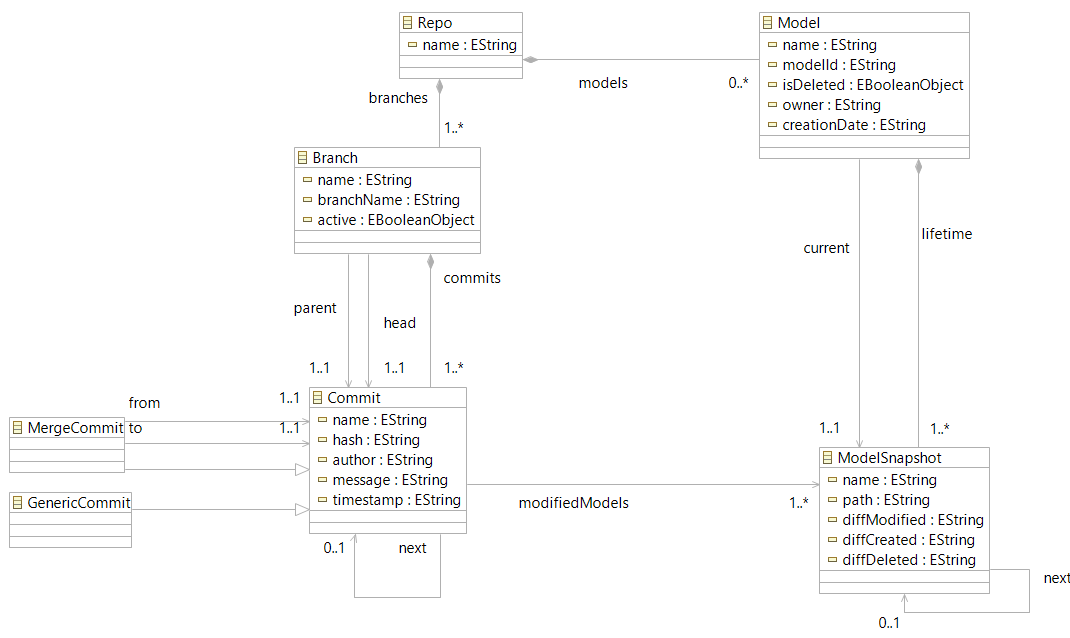
\includegraphics[width=\textwidth]{repomm.png}
  \caption{Métamodèle d'un Projet Versionnable}
  \label{fig:repomm}
\end{figure*}

Afin d'interroger le VCS sur un projet versionnable, il est nécessaire de
déterminer à priori les unités versionnables d'un projet. Cela est décrit dans
le métamodèle d'un projet versionnable présenté à la Figure \ref{fig:repomm}. Un
projet versionnable a une structure assez similaire à celle des projets
utilisant un VCS linéaire. Un projet consiste en des branches. Les branches
contiennent des commits définissant un point où l'on désire enregistrer des
changements. Les modèles constituent ici l'unité dont l'expert du domaine
modifiera dans le projet MDE. Chaque modèle possède une durée de vie exprimée
sous forme d'une série de snapshots.

\subsection*{Model Query Language - MQL}

\begin{figure}[ht!]
  \centering
  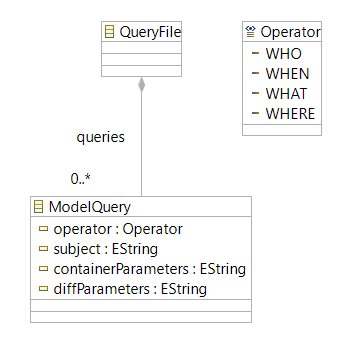
\includegraphics[width=0.4\textwidth]{mqlmm.png}
  \caption{Métamodèle de MQL}
  \label{fig:mqlmm}
\end{figure}

La syntaxe abstraite du langage MQL est exprimé dans le métamodèle de MQL à la
Figure \ref{fig:mqlmm}. Une expression MQL est constituée de plusieurs requêtes.
Chaque requête est composée d'un opérateur, du sujet de requête, et de
paramètres pour mieux filtrer les résultats attendues. La syntaxe concrète de ce
langage a été définie à l'aide de Xtext. Le Listing \ref{lst:mqlsyn} démontre un
exemple d'expression MQL. Dans cette expression, on remarque que chaque requête
est séparée par une virgule et que la dernière requête se termine par un point
d'interrogation. Chaque requête commence par un opérateur. La seconde requête
utilise l'opérateur \texttt{DESCRIPTION} qui s'agit ici tout simplement de sucre
syntaxique pour l'opérateur \texttt{WHERE} qui a été jugé ne pas être très
intuitif dans ce contexte.

\begin{lstlisting}[style=mql, label=lst:mqlsyn, caption=Expression MQL]
  WHO head {
    branchName = "main",
    active = "true"
  },
  DESCRIPTION parent {
    branchName = "b1"
  },
  WHEN created {
    timestamp < "2022-09-04"
  } [
    "MyDomainSpecificObject.x = 19"
  ]?
\end{lstlisting}

Un parseur Xtend a été implémenté pour produire un modèle MQL à partir d'une
expression MQL. Ce dernier génère un modèle MQL conforme au métamodèle MQL
lorsque l'expert du domaine sauvegarde le fichier où il rédigeait ses requêtes
MQL.

\subsection*{Transformations Modèle-à-texte}

À partir d'un modèle d'un projet versionnable conforme à son métamodèle, il est
ensuite possible de l'utiliser comme entrée à une transformation modèle-à-texte
qui produit une requête Cypher correspondante au modèle donné. Dans le cas d'un
projet versionnable, une requête pour créer une base de données de graphes est
générée à partir d'un modèle de projet versionnable.

À partir d'un modèle d'une expression MQL conforme à son métamodèle, une autre
transformation modèle-à-texte se sert de ce modèle comme entrée pour générer la
requête Cypher correspondante pour interroger la base de données existante du
projet versionnable. En prenant comme exemple la requête décrite au Listing
\ref{lst:mqlsyn}, après que le parseur Xtend aie généré le modèle MQL conforme
au métamodèle MQL, lorsque ce modèle est pris comme entrée à la transformation
modèle-à-texte, on obtient la requête Cypher décrite au Listing
\ref{lst:mqlegl}.

\begin{lstlisting}[style=cypher, label=lst:mqlegl,caption=Cypher générée]
  MATCH (b1:Branch)-[h1:head]->(c1:Commit)
  WHERE b1.branchName = "main" AND b1.active = "true"
  RETURN c1.author;
  MATCH (b2:Branch)-[p1:head]->(c2:Commit)
  WHERE b2.branchName = "b1"
  RETURN c2.message;
  MATCH (c3:Commit)-[mm1:modifiedModels]->(ms1:ModelSnapshot)
  WHERE c3.timestamp < "2022-09-04" AND "MyDomainSpecificObject.x = 19" IN ms1.diffCreated
  RETURN c3.timestamp;
\end{lstlisting}

\subsection*{Automatisation}

Afin d'automatiser le processus de création de base de données à partir d'un
projet versionnable et de traduction de la requête MQL pour ensuite afficher les
résultats de la requête, un Ant Workflow a été implémenté décrivant les étapes
du framework. La Figure \ref{fig:wfoutline} décrit les différentes étapes de
celui-ci.

\begin{figure}[ht!]
  \centering
  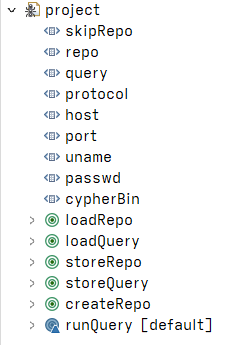
\includegraphics[width=0.3\textwidth]{wfoutline.png}
  \caption{Outline du Workflow}
  \label{fig:wfoutline}
\end{figure}

Il est possible de configurer certaines propriétés avant de démarrer le
workflow. La propriété \texttt{skipRepo} agit comme booléen décrivant si l'on
désire ne pas créer la base de donnée (dans le cas où elle a déjà été créée).
Les propriétés \texttt{repo} et \texttt{query} réfère aux noms de fichiers des
modèles du projet versionnable et de la requête qui seront utilisées comme
entrée aux transformations modèle-à-texte. Les propriétés \texttt{protocol},
\texttt{host}, \texttt{port}, \texttt{uname}, et \texttt{passwd} représentent
les valeurs pour se connecter à la base de donnée de graphes où l'on veut
entreprendre nos requêtes. La propriété \texttt{cypherBin} représente le chemin
de l'exécutable \texttt{Cypher} qui permettra de rouler des requêtes dans la
base de données. Le workflow est constitué de tâches à effectuer. Les tâches
\texttt{loadRepo} et \texttt{loadQuery} ne font que simplement charger le modèle
du projet versionnable et du modèle de la requête MQL respectivement. Les tâches
\texttt{storeRepo} et \texttt{storeQuery} appliquent la transformation
modèle-à-texte sur les modèles chargés. La tâche \texttt{createRepo} initialise
la base de donnée à partir de la requête Cypher généré du modèle de projet
versionnable. La tâche \texttt{runQuery} exécute la requête Cypher générée à
partir du modèle MQL et affiche les résultats.

\section*{Résultats obtenus}

Pour décrire les résultats obtenus, je vais présenter un exemple d'utilisation.
Considérant en premier lieu, le métamodèle d'une salle à manger. La Figure
\ref{fig:drmm} illustre le métamodèle en question. Il s'agit d'un simple
métamodèle décrivant la relation entre des tables et des chaises dans une
salle. Nous supposerons que l'expert du domaine conçoit un projet de salle à
manger. 

\begin{lstlisting}[style=mql,label=lst:mqldr1, caption=Exemple d'expression MQL]
  WHAT head {
    branchName = "main"
  }?
\end{lstlisting}

La figure \ref{fig:repom} décrit l'état du projet versionnable de notre expert
du domaine sous forme de modèle conformant au métamodèle de projet
versionnable. Celui-ci s'agit d'un projet assez simple contenant 3 modèles de
salle à manger, 2 branches et 6 commits au total. On a par la suite comme
exemple de requête celle présentée au Listing \ref{lst:mqldr1}. On peut
maintenant exécuter le workflow qui commence par génèrer les requêtes Cypher
appropriées, initalise la base de donnée, et exécute la requête Cypher obtenue
de la transformation modèle-à-texte du modèle MQL pour obtenir les résultats de
la Figure \ref{fig:res1}.

\begin{figure}[ht]
  \centering
  \begin{minipage}{0.5\textwidth}
    \centering
    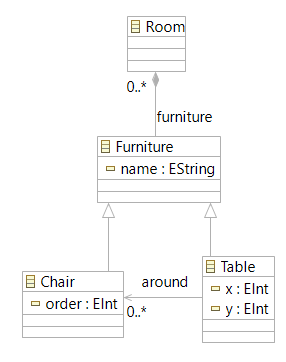
\includegraphics[width=0.4\linewidth]{drmm.png}
    \captionof{figure}{Métamodèle d'une salle à manger}
    \label{fig:drmm}
  \end{minipage}%
  \begin{minipage}{0.5\textwidth}
    \centering
    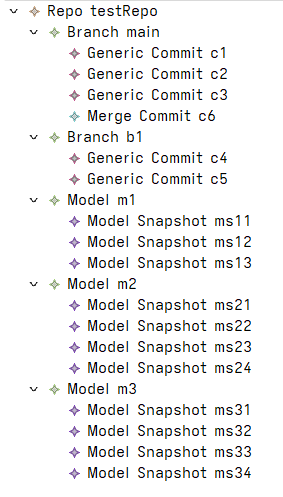
\includegraphics[width=0.4\linewidth]{repom.png}
    \captionof{figure}{Modèle de Projet Versionnable}
    \label{fig:repom}
  \end{minipage}
\end{figure}

\begin{figure}[ht!]
  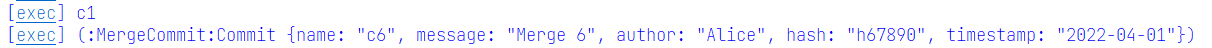
\includegraphics[width=\textwidth]{res1.png}
  \caption{Résultat de la première requête}
  \label{fig:res1}
\end{figure}

Considérant maintenant la requête au Listing \ref{lst:mqldr2}. Puisque nous
avions déjà généré la base de données de graphes de notre projet versionnable,
on s'assure de mettre la propriété \texttt{skipRepo} à \texttt{true} avant de
démarrer le workflow.

\begin{lstlisting}[style=mql,label=lst:mqldr2,
  caption=MQL Expression specific to Dining Room domain]
  WHERE model {
    owner = "Philippe"
  },
  WHEN changed [
    "MyTable.x = 3"
  ]?
\end{lstlisting}

En exécutant le workflow après avoir bien définit les valeurs des propriétés, on
obtient le résultat illustré à la figure \ref{fig:res2}.

\begin{figure}[h]
  \centering
  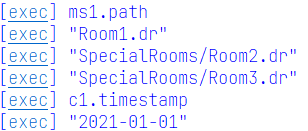
\includegraphics[width=0.3\textwidth]{res2.png}
  \caption{Résultat de la seconde requête}
  \label{fig:res2}
\end{figure}

\section*{Améliorations futures}

En conclusion, j'ai présenté un langage de requête spécifique au domaine de
projets versionnables pour interroger un projet versionnable sous un domaine
spécifique. J'ai également présenté un framework décrivant comment les
différentes composantes du projet interagissent entre elles. Il a été nécessaire
de définir les unités versionnables d'un projet à l'aide du métamodèle d'un
projet versionnable et de définir les transformations modèle-à-texte nécessaire
pour générer les requêtes Cypher pour interagir avec la base de données Neo4j.

En tant que travaux futurs, je prévoie ajouter un meilleur support pour la
fonctionnalité d'autocomplétion offerte par Xtext au moyen d'être capable
d'accéder au contenu d'un modèle existant. Un tel ajout ferait en sorte que les
paramètres \texttt{diff} au sein d'une expression MQL ne sont plus fournis en
tant chaînes de caractères littérales mais des références aux éléments existants
du modèle spécifique au domaine dans le projet. Il permettrait également la
validation de requêtes impliquant des paramètres \texttt{diff}.

De plus, je prévoie améliorer l'expressivité des requêtes MQL. À l'heure
actuelle, des requêtes de base peuvent être effectuées en utilisant les
différents opérateurs fournis. Il serait intéressant de permettre des requêtes
plus complexes, basées sur une séquence de commits par exemple, ou fournissant
des analyses statistiques.

Présentement, l'outil de workflow n'est disponible que dans Eclipse. Le
possibilité d'invoquer l'outil en tant qu'utilitaire de ligne de commande, ou un
fichier jar, ou même un un plugin Eclipse serait préféré pour donner
l'opportunité qu'il soit intégré aux flux de travail existants. Pour ce faire,
il faudrait regrouper les composantes et y inclure les dépendances appropriées
pour l'exécution indépendante de EMF.

La mise en oeuvre d'un parseur de projet versionnable est une idée intéressante
dans le contexte de l'inclusion d'une telle une étape dans le
framework. Considérant un projet versionnable existant spécifique au domaine,
qu'il soit géré par des VCS orientés ligne tels que git ou non, il serait
souhaitable de générer le modèle de projet versionnable correspondant conforme
au métamodèle de projet versionnable.

Le Neo Modeling Framework (NMF) \cite{nmf} est un ensemble d'outils open-source
conçu pour manipuler des ensembles de données ultra-volumineux dans la base de
données Neo4j. Il comprend un chargeur qui a la capacité de charger un modèle
Ecore et de produire une base de données de graphes. Il fournit également un
générateur qui peut générer une API spécifique au domaine pour modifier un
modèle spécifique. Intégrer le workflow lors de l'utilisation du MQL avec NMF
pourrait fournir divers atouts. L'intégration avec NMF et la comparaison avec le
flux de travail actuel est une idée future qui pourrait aider à mieux orienter
les idées de ce projet.

L'intégration avec DSMCompare \cite{dsmcompare} est un autre atout souhaitable à
considérer. Par exemple, il pourrait être possible d'interroger les différences
sémantiques entre les modèles d'une expression MQL et récupérer le
\texttt{diff\_model} à partir de DSMCompare sur lequel plus de requêtes peuvent
être exprimées.

\bibliographystyle{plain} 
\bibliography{refs}

\end{document}

